\documentclass{article}
\usepackage{gvv-book}
\usepackage{gvv}
\usepackage{amsmath}
\usepackage{amsfonts}
\usepackage{tikz}
\usepackage{setspace}
\usepackage{gensymb}
\usepackage[cmex10]{amsmath}
\usepackage{amsthm}
\usepackage{mathrsfs}
\usepackage{txfonts}
\usepackage{stfloats}
\usepackage{bm}
\usepackage{cite}
\usepackage{cases}
\usepackage{subfig}
\usepackage{longtable}
\usepackage{multirow}
\usepackage{enumitem}
\usepackage{mathtools}
\usepackage{tikz}
\usepackage{circuitikz}
\usepackage{verbatim}
\usepackage[breaklinks=true]{hyperref}
\usepackage{tkz-euclide}
\usepackage{listings}
\usepackage{color}    
\usepackage{array}    
\usepackage{longtable}
\usepackage{calc}     
\usepackage{multirow} 
\usepackage{hhline}   
\usepackage{ifthen}   
\usepackage{lscape}     
\usepackage{chngcntr}
\usepackage{graphicx}
\usepackage{float}
\usepackage{multicol}
\usepackage[a4paper, left = 1.5cm, right = 1.5cm]{geometry}

\begin{document}

\begin{center}
\large
    \textbf{Samyak Gondane-AI25BTECH11029}
\end{center}
\date{}

\section*{Question}
Find the equation of the circle passing through $(0, 0)$ and making intercepts $a$ and $b$ on the coordinate axes.


\section*{Solution}

Let:
\begin{align}
\vec{x_1} = \myvec{0 \\ 0},\ \vec{x_2} = \myvec{a \\ 0},\ \vec{x_3} = \myvec{0 \\ b}
\end{align}

We use the general matrix form of a circle:


\begin{align}
\myvec{2x_1 & 2x_2 & 2x_3\\
1 & 1 & 1}^T \myvec{\vec{u} \\ f} = - \myvec{\norm{x_1}^2 \\ \norm{x_2}^2 \\ \norm{x_3}^2}
\end{align}


\begin{align}
\myvec{
2x_1^T & 1 \\
2x_2^T & 1 \\
2x_3^T & 1
}
\myvec{
\vec{u} \\
f
}
=
- \myvec{
\norm{x_1}^2 \\
\norm{x_2}^2 \\
\norm{x_3}^2
}
\end{align}


Substituting the values:

\begin{align}
\myvec{
0 & 0 & 1 \\
2a & 0 & 1 \\
0 & 2b & 1
}
\myvec{
u_1 \\
u_2 \\
f
}
=
- \myvec{
0 \\
a^2 \\
b^2
}
\end{align}


Solving the system:

\begin{align*}
f &= 0 \\
2a u_1 + f &= -a^2 \Rightarrow u_1 = -\frac{a}{2} \\
2b u_2 + f &= -b^2 \Rightarrow u_2 = -\frac{b}{2}
\end{align*}

\subsection*{Final Result}

\begin{align}
\vec{u} = \myvec{ -\frac{a}{2} \\ -\frac{b}{2} }, \quad f = 0
\end{align}


So the equation of the circle becomes:


\begin{align}
x^2 + y^2 + ax + by = 0
\end{align}


\begin{figure}[H]
    \centering
    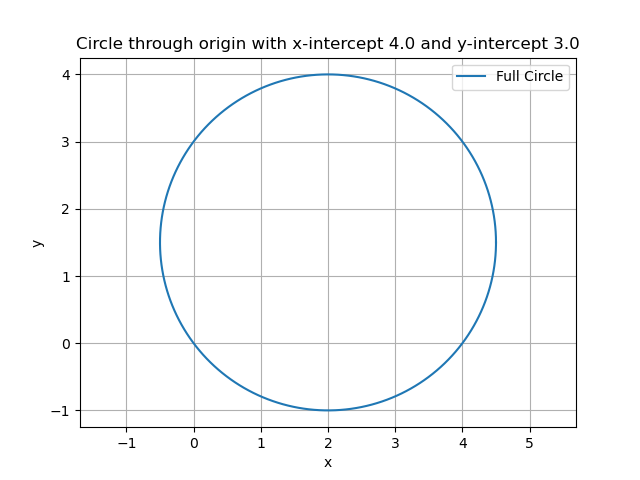
\includegraphics[width=0.7\linewidth]{./figs/Figure_1.png}
    \caption{}
    \label{fig:fig1}
\end{figure}

\end{document}